%%%%%%%%%%%%%%%%%%%%%%%%%%%%%%%%%%%%%%%%%%%%%%%%%%%%%%%%%%%%%%%%%%% 
%                                                                 %
%                            CHAPTER                              %
%                                                                 %
%%%%%%%%%%%%%%%%%%%%%%%%%%%%%%%%%%%%%%%%%%%%%%%%%%%%%%%%%%%%%%%%%%% 

\chapter{Software implementation of the Smith-Waterman algorithm}
\label{ch:SoftwareImpl}

This chapter will cover an approach to genome mapping using the Smith-Waterman algorithm. This is a computationally very demanding task, but is more precise than heuristic methods such as FASTA and BLAST.

\section{The concept}
For genome mapping a sequence of 75 to 300 bases in length should be mapped to the reference genome. The idea behind this mapping and the applications is thoroughly described in chapter \ref{ch:algoverzicht}.

In this implementation, a mapping with "pure" Smith-Waterman was chosen. For sequencing applications where only a small part of the genome is sequenced, the read should only be mapped to these small candidate locations. The most computationally demanding task is when the alignment should be done with the whole genome. In this thesis, the alignment of the sequence is done with the whole genome. However, the concept is also applicable for read alignment to a selected region of a genome or a set of genomes from different organisms.

\begin{figure}[H]
	\centering
	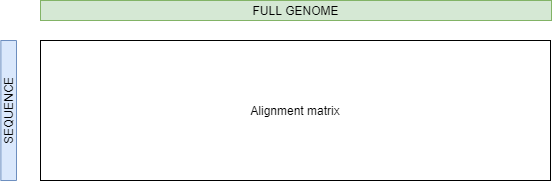
\includegraphics[width=0.6\textwidth]{systemImplementation/pureSWconcept.png}
	\caption{The concept of the implementation: the sequences is mapped to the whole genome}
	\label{fig:concept}
\end{figure}


\section{General overview of the implementation}

\subsection{Parameters and Types}

\paragraph{Nucleotide base}
First of all, it seemed important to define the nucleotide bases. There are only 4 possible bases ($A$, $C$, $G$ and $T$), so 2 bits are enough. The following coding was chosen:

\begin{table}[H]
	\centering
	\begin{tabular}{|l|c|c|c|c|}
		\hline
		\textbf{Base} & A  & C  & G  & T  \\ \hline
		\textbf{Code} & 00 & 01 & 10 & 11 \\ \hline
	\end{tabular}
	\caption{\centering Encoding for the nucleotide bases}
\end{table}

To store these bases the uint8\_t type from the stdint library was used. It is 1 byte in size which is the smallest available type in the C language. If more time would have been available, and an implementation with the full human genome would have been made, it might be a good idea to define a specific type consisting of only 2 bits, which would be a lot more memory efficient.

\paragraph{DNA sequence type} To easily keep track of a sequence in the program, a type was created which can hold a sequence of DNA. It consists of 2 parts: the length of the sequence and a pointer to the first base in memory. 
Since the genome can have a length of more than 3 billion bases, and the sequence is only a maximum of 300 bases in length, it made sense to use a separate type for the reference and the sequence.\\

\begin{figure}[H]
	\centering
	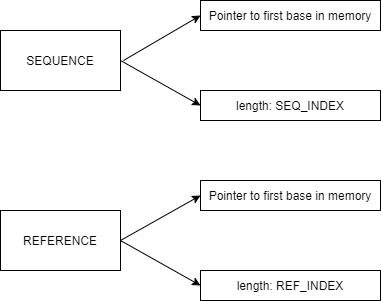
\includegraphics[width=0.35\textwidth]{systemImplementation/RefAndSeqTypes.png}
	\caption{The created types to store the sequence and the reference}
	\label{fig:RefAndSeqTypes}
\end{figure}

To index these "arrays" of bases, a new type was created for both the sequence indexing (\emph{SEQ\_INDEX}) and the reference indexing (\emph{REF\_INDEX}). Since an index to the sequence can be as high as the $length - 1$, it made sense to make the length attribute out of these newly created index types.

\subsection{The code structure}

\begin{enumerate}
	\item Allocate some memory for the following data:
	\begin{enumerate}
		\item The reference genome, which can be quite large;
		\item current read;
		\item reverse complementary of current read;
		\item matrix for during the alignment. The amount of memory that should be allocated to this matrix is equal to the size of the sequence times the size of the reference.
	\end{enumerate}
	\item Initialize the first row and first column of the matrix on $0$, to prevent edge cases when performing the Smith-Waterman Algorithm;
	\item Load the reference genome from the fasta file;
	\item Open the FASTQ file for loading unmapped reads, and the SAM file to store the reads once they are mapped;
	\item For every read in the FASTQ file, we perform the following operations:
	\begin{enumerate}
		\item Load the next read from FASTQ file;
		\item Perform the alignment. (see \ref{expl:alignment});
		\item write the mapped read to the SAM file;
	\end{enumerate}
	\item Close the FASTQ and SAM files;
	\item free the reserved memory again
\end{enumerate}

\section{Details of the implementation}

As in most implementations in software, it was decided to split up the functionality of the program in multiple blocks. We have 3 big blocks:
\begin{enumerate}
	\item Interfacing with the memory: reserving memory for the reference, the sequence, and the alignment matrix.
	\item Interfacing with the files and the filesystem: Since the FASTA, FASTQ and SAM files are in a specific format, it made sense to build interpreters from and to these formats. 
	\item The alignment itself, which is the core of the program.
\end{enumerate}

\begin{figure}[H]
	\centering
	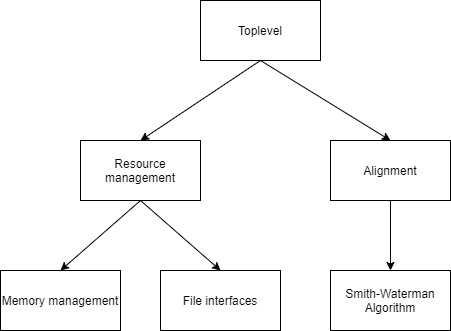
\includegraphics[width=0.5\textwidth]{systemImplementation/organigram.png}
	\caption{An organisation chart of the split up functionalities}
	\label{fig:organigram}
\end{figure}

\subsection{File interfaces}

\subsubsection{Parameters and types}

Since we need to interface FASTA, FASTQ, and SAM files, it seemed appropriate to create 3 custom types. For the FASTA file, which stores the genome, the type \emph{GENOME} was created. In the case of the FASTQ file and the SAM file, the respective types \emph{READ} and \emph{MAPPED\_READ} were created. Notice that the attributes of the types match the information to interface the files.

The information stored in the \emph{GENOME} type is the name of the genome (\emph{Rname}) and the reference.

\begin{figure}[H]
	\centering
	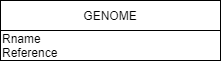
\includegraphics[width=0.35\textwidth]{systemImplementation/GenomeType.png}
	\caption{The type created to store the genome information.}
	\label{fig:GenomeType}
\end{figure}

In the \emph{READ} type, the current sequence is stored together with its quality string and its name.

\begin{figure}[H]
	\centering
	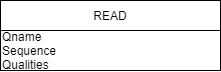
\includegraphics[width=0.35\textwidth]{systemImplementation/ReadType.png}
	\caption{The type created to store the read information}
	\label{fig:ReadType}
\end{figure}

The \emph{MAPPED\_READ} type contains all the information needed to write a full line in the SAM file, which is the output of the program.
Mark, the read itself is also stored in this type since all the information in the read will also be written to the SAM file.

\begin{figure}[H]
	\centering
	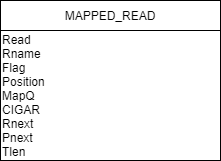
\includegraphics[width=0.35\textwidth]{systemImplementation/mappedReadType.png}
	\caption{The type created to store the mapping information, together with the read}
	\label{fig:mappedReadType}
\end{figure}

\subsubsection{Code structure}
\label{codeStructure}

First of all, the representation of the bases in the files (which is in the ASCII character format) should be transformable to the BASE type in the program. Because of this, conversion functions were created to change the character to base or vice versa.

\paragraph{FASTA interface} The function of this part is to load the genome from the FASTA file into the created \emph{GENOME} type. 
The FASTA file format is a simple text-based way of storing a genome. On the first line is a '>' character followed by the name of the genome (\emph{Rname}). Starting from the second line to the end of the file the genome is stored. Often, this genome is split up using spaces or in multiple lines, so when coding the interpreter we need to make sure to skip these whitespace characters.

For better code readability, the genome loading is split into 2 functions that are executed in order:
\begin{enumerate}
	\item loading the genome info
	\item loading the genome into the REFERENCE type. 
\end{enumerate}

\paragraph{FASTQ interface} this part of the program is responsible for loading the next read as a stream. The buildup of a FASTQ file is thoroughly described in \ref{expl:FASTQ}.

In this case, the code was also split up into functions for better readability:
\begin{enumerate}
	\item Loading the QName, which is found on the first line for every read, behind a '@' character
	\item Loading the sequence, which is stored in a text-based format in the FASTQ file, so it should be transformed to the SEQUENCE type. In a sequence, a base may be suddenly marked with an 'N' character, which means after the primary processing the process was unable to identify the base. Because of the way the sequencing machines work, this mostly happens at the end of the sequence. So, it was decided to only cut the sequence short at the moment an 'N' character is registered.
	
	For example, if the sequence were $ACGGCGCATTACNNAN$, the interface will only store $ACGGCGCATTAC$. This is justified by the fact that we are statistically certain that this sequence will be matched correctly from the moment the read is more than 15-20 bases long. The statistical proof itself will not be covered in this thesis.
	\item loading the qualities. Found on the fourth line for each read, the qualities for each base are stored. The information is stored in an array with the same length as the sequence.
	
\end{enumerate}


\paragraph{SAM interface} The SAM interface will write the current mapped read to a SAM file, one line for one read. The buildup of a SAM file is thoroughly described in \ref{expl:SAM}.

For this implementation, some values of the SAM format are not important and should be set to a default value. So it came naturally to create an "init" function, in which these default values are assigned. 
\begin{itemize}
	\item RNext should be set to the '*' character;
	\item Pnext should be set to 0;
	\item TLen should be set to 0;
\end{itemize}

Then, to write the line in the output SAM file, a function was created which accepts an attribute of the \emph{MAPPED\_READ} format and writes it as a line in the file.

\subsection{Memory management}

\subsubsection{malloc and sds\_alloc}
The allocation of memory in a C program is usually done using the "malloc" function. However, on the used SoC, a distribution of Linux is running. Like in most operating systems, this Linux distribution uses a virtual address space to enlarge the available RAM virtually. 

The original idea for the project was to be able to accelerate certain functions using the programmable hardware available in the SoC chip. Since this hardware should be able to access the data in the memory, there two options:
\begin{enumerate}
	\item Build a copy of the address translator on the hardware. This would require a lot of work and would slow the whole process of looking things up in memory down.
	\item Let the software interface the physical memory so that we don't use the virtual addresses. This solution was used in the final implementation
\end{enumerate}

Luckily, Xilinx has published a library with an \emph{sds\_alloc} function. This does the same as the malloc function in the C language but in physical memory instead of the virtual memory.

\subsubsection{Allocating memory}
To allocate memory, the following formula was used:

\begin{lcverbatim}
	memory_pointer = (TYPE*) sds_alloc( length * sizeof(TYPE) );
\end{lcverbatim}

The sds\_alloc function returns a pointer to the first address in memory that has been reserved. It turns out that this pointer should be cast explicitly to the type used.

\begin{itemize}
	\item In case of reserving space for the sequence and the reference, the "TYPE" part in the formula should be filled in by the BASE type. For the length part of the formula, parameters were created named seqMax and refMax respectively.
	\item When space for the alignment matrix will be reserved, the "TYPE" part in the formula should be filled in by the CELL type (for more explanation on the CELL-type, see \ref{expl:AlignmentParams}). As for the length of the space to reserve, this should be equal to refMax times seqMax.
\end{itemize}

\subsection{The alignment}
\label{expl:alignment}

\subsubsection{Parameters and types}
\label{expl:AlignmentParams}

A naive approach to implementing the S-W algorithm might be to have the alignment matrix filled in by the values only. If we would use this approach, it would quickly become clear that the backtracking is impossible, since we also need to know where the value originates from. Also, when generating the CIGAR-string, it is good to know which direction it originates from, as it implies a match (M), insertion (I), or a deletion (D). Since all this information should be stored in the alignment matrix, it seemed a good idea to create a new type. This type was called \emph{CELL}.

\begin{figure}[H]
	\centering
	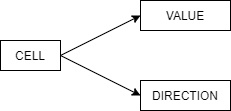
\includegraphics[width=0.35\textwidth]{systemImplementation/CellType.png}
	\caption{The type created to store the information for every cell in the alignment matrix}
	\label{fig:CellType}
\end{figure}

The cell stores the place it originates from, using a \emph{DIRECTION} attribute. There are 4 possible directions a value can originate from: zero (coded as 0), diagonal (1), up (2), left (3).

Furthermore, it stores the value using a special type \emph{CELL\_VALUE}. The size of values this type can store should be greater than the length of the sequence times the similarity score. Keep in mind that to calculate the maximum, this value-type should be able to go negative.

\subsubsection{Code structure}

\paragraph{The alignment layer}

The alignment layer does everything in the alignment of the sequence that has nothing to do with the matrix fill in. That functionality is outsourced to a separate function.

Also, for the CIGAR string, a certain threshold was programmed in. The CIGAR string of a matched read consists of multiple parts. For example: $6M1I7M$ consists of 3 parts; $6M$, $1I$ and $7M$. By limiting the number of parts that are allowed we can define a threshold by which a sequence is considered as "aligned". If both the forward and reverse sequences go over this limit, the sequence will be marked as "unmatched".

\begin{enumerate}
	\item Fill in the matrix using the forward direction of the sequence.
	\item Store the maximum value of the matrix.
	\item Generate the CIGAR string for this forward direction. We have to do this so early because you need the full matrix for the CIGAR generation, and we want to reuse the memory for the matrix according to the reverse sequence.
	\item Check if the CIGAR limit has been exceeded. If not, then store the position of the map. 
	\item Reverse the sequence
	\item Repeat for the reverse sequence.
	\item Check for the limit of the CIGAR. If it was exceeded in both forward and reverse sequence, mark it as unmatched.
	\item Check which read fit best (the forward or reverse one) by comparing the maximum values in the mapping. Assign the best one to the MAPPED\_READ type.
\end{enumerate}

\paragraph{The fill in layer}
This is probably the easiest layer of them all, but will also be one of the most computationally demanding ones. It skims over every cell in the matrix, except for the first row and first column, and uses the cell generation layer to generate the cell on that specific spot. Also, while having an iteration that goes over every cell, it is a good idea to use this iteration to find the maximum cell in the matrix, which is the starting point for the backtracking.

\paragraph{The cell generation layer}
This layer consists of 3 parts:
\begin{enumerate}
	\item Generate the 3 values originating from diagonal, up, and left cells, using the formulas described by the S-W algorithm. For this step, the parameters $s$ (for the similarity score) and $gp$ (for the gap penalty) were created. For testing, These were mostly kept on $s=3$ and $gp=2$, but can be easily changed according to one's needs.
	\item Determine which of these three values is the greatest. If all negative, choose 0.
	\item Assign the correct value and direction of the newly generated cell.
\end{enumerate}

This layer must be efficiently coded, and since it runs for every cell (and there are a lot of cells), it can be expected to be the core of the program.

\section{Implementation results}

\subsection{The IGV software}

The free and easy to download program IGV\cite{12} %cit
(or Integrative Genomics Viewer) is a visualization tool for exploring genomic datasets. In practice, it is used to examine the results from mapped reads.

\begin{figure}[H]
	\centering
	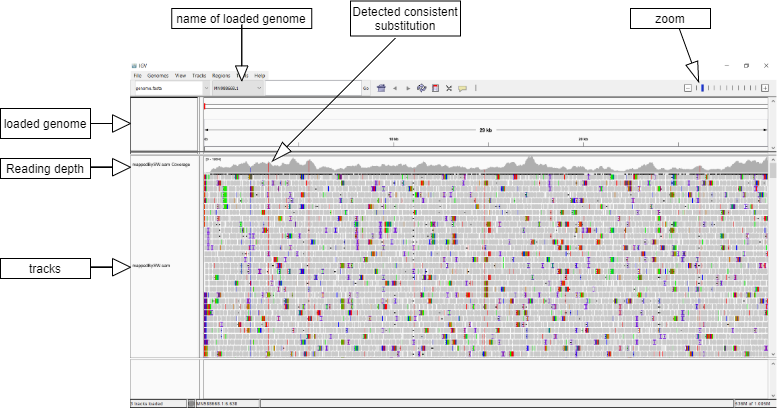
\includegraphics[width=\textwidth]{softwareResults/IGVlayout.png}
	\caption{The layout of the IGV analysing software}
	\label{fig:IGVlayout}
\end{figure}

The most important functions in IGV for this thesis are: 
\begin{itemize}
	\item It color-codes insertion, deletions or substitutions, so it is easy to see "from a distance";
	\item It can display the read depth for every base in the genome;
	\item If the read depth is sufficient, it can also determine if an indel or substitution is part of the read, or is consistent enough throughout all the reads to show it in the full genome;
	\item The sequence direction is indicated by an arrow when examining a specific read.
\end{itemize}

\begin{figure}[H]
	\centering
	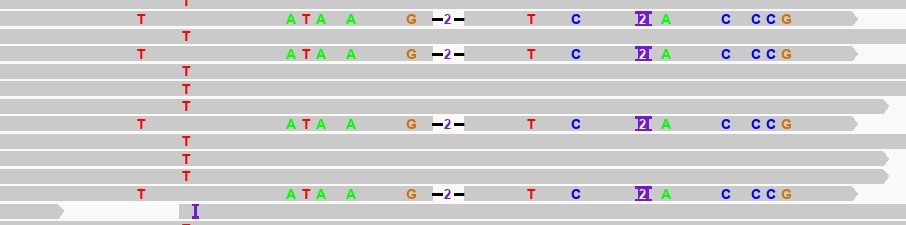
\includegraphics[width=0.8\textwidth]{softwareResults/IGVcloseup.jpg}
	\caption{Close-up of a few reads in the IGV analysing software. Notice how the color coded bases are substitutions, whereas the matched bases are not shown. Moreover, a gap and insertion is also visible}
	\label{fig:IGVcloseup}
\end{figure}

\subsection{Sample data}

To try the implementation on the human genome directly seemed way too ambitious. Therefore, it seemed appropriate to try the implementation first on an organism that has a genome of only a few thousand bases in length.
Since this thesis is performed around the spring of 2020, the "coronavirus" (or SARS-CoV-2) seemed like an appropriate candidate. After a quick google search, it turned out that this virus had a genome consisting of merely 29 thousand bases.

The genome of the coronavirus was found easily online with reference number MN988668.1 in the genome bank of NCBI.\cite{11}

The FASTQ files obtained from a DNA sequence for the coronavirus used in this thesis were found in the SRA (sequence read archive) of the NCBI, submitted by the University of Washington.\cite{NCBI}
%src: https://www.ncbi.nlm.nih.gov/sra/SRX7852918

Of course, when fitting these fastQ files through the implementation from this thesis, we have to be able to compare it with an implementation which is considered as correct. Therefore, an online tool (galaxy) was used where a lot of existing bioinformatical algorithms and programs can be performed on given sample data using cloud computing.\cite{13} %src ook zetten naar galaxy
By converting the fastQ files (given by the SRA of the NCBI) using one of these available applications, we can get a pretty good reference to match our results against. As the application to compare to, the Bowtie 2 algorithm was chosen, which is based on the S-W algorithm.

\subsection{Results}

We will compare the results from the sample data using the online Bowtie application and the implementation described in this chapter.

After running the software implementation overnight with the unmapped sequences from the coronavirus, we obtained a dataset of mapped reads. Both these mapped reads and the dataset obtained by using the Galaxy online tool were imported into IGV for comparison, which can be seen in figure \ref{fig:IGVcomparison}

\begin{figure}[H]
	\centering
	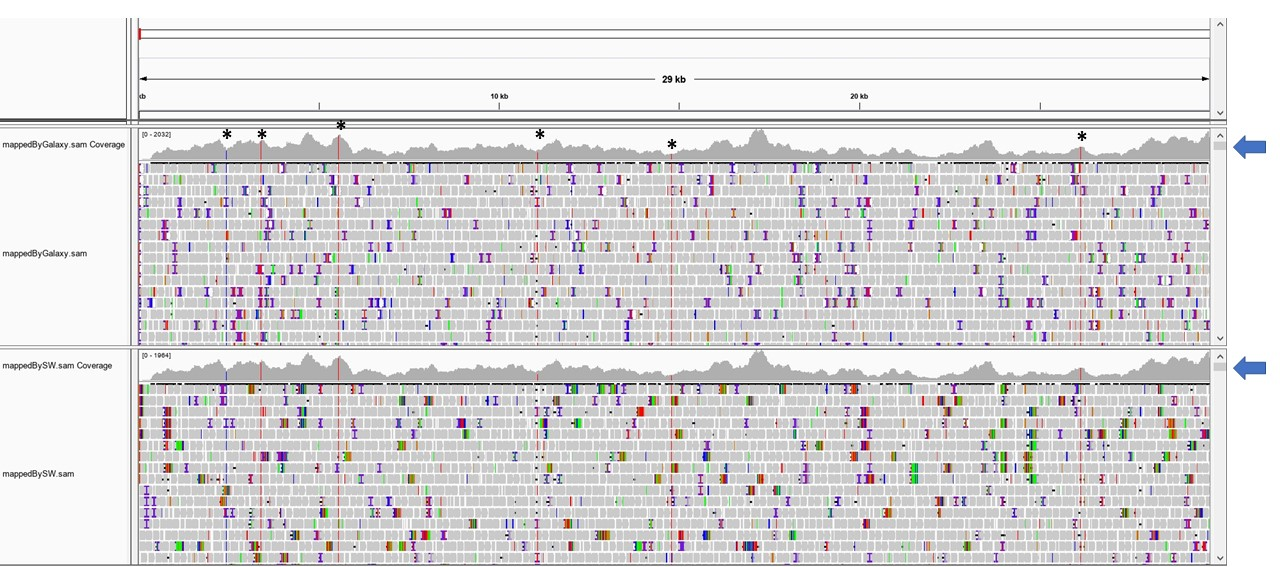
\includegraphics[width=\textwidth]{softwareResults/comparison.jpg}
	\caption{A comparison of the data obtained by Galaxy (top) and the data obtained by the implementation discussed in this chapter (bottom)}
	\label{fig:IGVcomparison}
\end{figure}

It can be observed that the implementation is working correctly since the reading depth graphs are approximately the same (indicated by an arrow). Furthermore, IGV was able to detect and identify consistent substitutions or indels in the reads.

If you look closely to figure \ref{fig:IGVcomparison}, some small differences between the exact reads are visible. This will probably be because both the algorithm and the parameters were a bit different. However, the important part is that the reading depths are the same, as well as the consistently mutated bases marked in the genome (indicated by an asterisk).


\paragraph{The implications for the coronavirus data}
The coronavirus is constantly changing because of the mutations of some bases in the genome over time, just like the flu. In this way, it is possible to trace where infections originate. For example, the corona in China can have slightly different bases than from Italy or Spain. We can identify these changes by sequencing the whole genome and looking for consistent substitutions or indels over the whole dataset.

From these results shown by IGV \ref{fig:IGVcomparison}, some mutations are shown, so we can assume that the coronavirus which was sequenced in Washington (taken from a US patient, the FASTQ file used) has some slight differences with the original Chinese sequenced genome (the reference sequence).
